%====================================================
\section{Impact and Conclusion}

\begin{frame}{Anticipated Intake Workflow}
	\begin{center}
	\resizebox{0.92\textwidth}{!}{%
	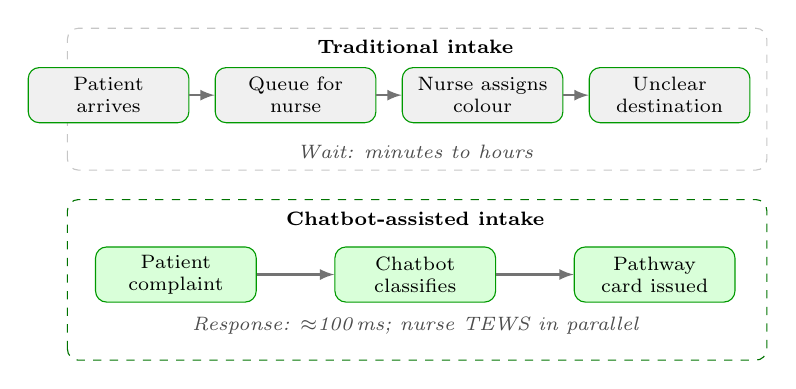
\begin{tikzpicture}[
	  x=0.95cm, y=0.68cm,
	  title/.style={font=\scriptsize\bfseries, anchor=center},
	  box/.style={draw=green!60!black, rectangle, fill=green!10, text width=1.9cm, align=center,
	    minimum height=0.7cm, rounded corners, font=\scriptsize, inner sep=2pt},
	  old/.style={box, fill=gray!12},
	  new/.style={box, fill=green!15},
	  arrow/.style={->, >=latex, thick, draw=black!55},
	  foot/.style={font=\scriptsize\itshape, text=black!70, align=center}]
	  \node[title] at (4.3, 6.2) {Traditional intake};
	  \draw[dashed, rounded corners, draw=gray!45] (-0.35, 3.9) rectangle (9.0, 6.55);
	  \node[old] (q) at (0.2, 5.3) {Patient\\arrives};
	  \node[old] (wait) at (2.7, 5.3) {Queue for\\nurse};
	  \node[old] (nurse) at (5.2, 5.3) {Nurse assigns\\colour};
	  \node[old] (unclear) at (7.7, 5.3) {Unclear\\destination};
	  \draw[arrow] (q) -- (wait);
	  \draw[arrow] (wait) -- (nurse);
	  \draw[arrow] (nurse) -- (unclear);
	  \node[foot] at (4.3, 4.25) {Wait: minutes to hours};
	  \node[title] at (4.3, 3.0) {Chatbot-assisted intake};
	  \draw[dashed, rounded corners, draw=green!45!black] (-0.35, 0.35) rectangle (9.0, 3.35);
	  \node[new] (c) at (1.1, 1.95) {Patient\\complaint};
	  \node[new] (bot) at (4.3, 1.95) {Chatbot\\classifies};
	  \node[new] (card) at (7.5, 1.95) {Pathway\\card issued};
	  \draw[arrow] (c) -- (bot);
	  \draw[arrow] (bot) -- (card);
	  \node[foot] at (4.3, 1.0) {Response: \(\approx\)100\,ms; nurse TEWS in parallel};
	\end{tikzpicture}}
	\end{center}
\end{frame}

\begin{frame}{Anticipated Impact}
	\begin{itemize}
		\item \textbf{Faster start:} the chatbot can suggest how urgent a patient is as soon as they describe their problem.
		\item \textbf{Safer for critical patients:} it is built to catch the most urgent cases so they are less likely to be missed.
		\item \textbf{Clearer next steps:} each colour comes with a short pathway card (where to go and what to do).
		\item \textbf{Nurses stay in charge:} the tool only assists; staff can check vitals and change the decision.
	\end{itemize}
\end{frame}

\begin{frame}{Selected References}
	\small
	\begin{enumerate}
		\item Lee et al.\ (2020). BioBERT for biomedical text mining. \emph{Bioinformatics}.
		\item Stewart et al.\ (2023). NLP at ED triage: a narrative review. \emph{PLOS ONE}.
		\item South African Triage Group (2012). \emph{SATS Training Manual}.
		\item Chawla et al.\ (2002). SMOTE: Synthetic Minority Over-sampling Technique.
		\item Laitinen-Fredriksson Foundation (2025). Triagegeist (Kaggle).
		\item Mitchell et al.\ (2023); Rominski et al.\ (2014); Berkowitz et al.\ (2019).
	\end{enumerate}
\end{frame}
